\documentclass[10pt,twocolumn,letterpaper]{article}

\usepackage{cvpr}
\usepackage{times}
\usepackage{epsfig}
\usepackage{graphicx}
\usepackage{amsmath}
\usepackage{amssymb}

% Include other packages here, before hyperref.

% If you comment hyperref and then uncomment it, you should delete
% egpaper.aux before re-running latex.  (Or just hit 'q' on the first latex
% run, let it finish, and you should be clear).
\usepackage[breaklinks=true,bookmarks=false]{hyperref}

\cvprfinalcopy % *** Uncomment this line for the final submission

\def\cvprPaperID{****} % *** Enter the CVPR Paper ID here
\def\httilde{\mbox{\tt\raisebox{-.5ex}{\symbol{126}}}}

% Pages are numbered in submission mode, and unnumbered in camera-ready
%\ifcvprfinal\pagestyle{empty}\fi
\setcounter{page}{1}
\begin{document}

%%%%%%%%% TITLE
\title{AFEW Competition of Emotion Recognition}

\author{Cao Kaidi\\
EE43\\
2014012282
\and
Lin Ji\\
EE43\\
2014011097
\and
Yan Jingkai\\
EE46\\
2014011192
}

\maketitle
%\thispagestyle{empty}

%%%%%%%%% ABSTRACT
\begin{abstract}
   This paper presents the implementation details of our video-based hybrid emotion recognition network. The proposed approach combines information from video frames and audios, which are processed separately. Video frames are first preprocessed with face detection units and aligned for regularization. AlexNet and LSTM are employed for video feature extraction and learning. For audio, we adopt a non-deep learning approach via SVM, applying OpenSmile for feature extraction. Finally, the output predition vectors of the two streams are synthesized and gives the final prediction.

   The model achieves a validation accuracy of $47.23\%$, while test accuracy is yet to be examined.
\end{abstract}

%%%%%%%%% BODY TEXT

\begin{figure*}[htpb]
	\centering
	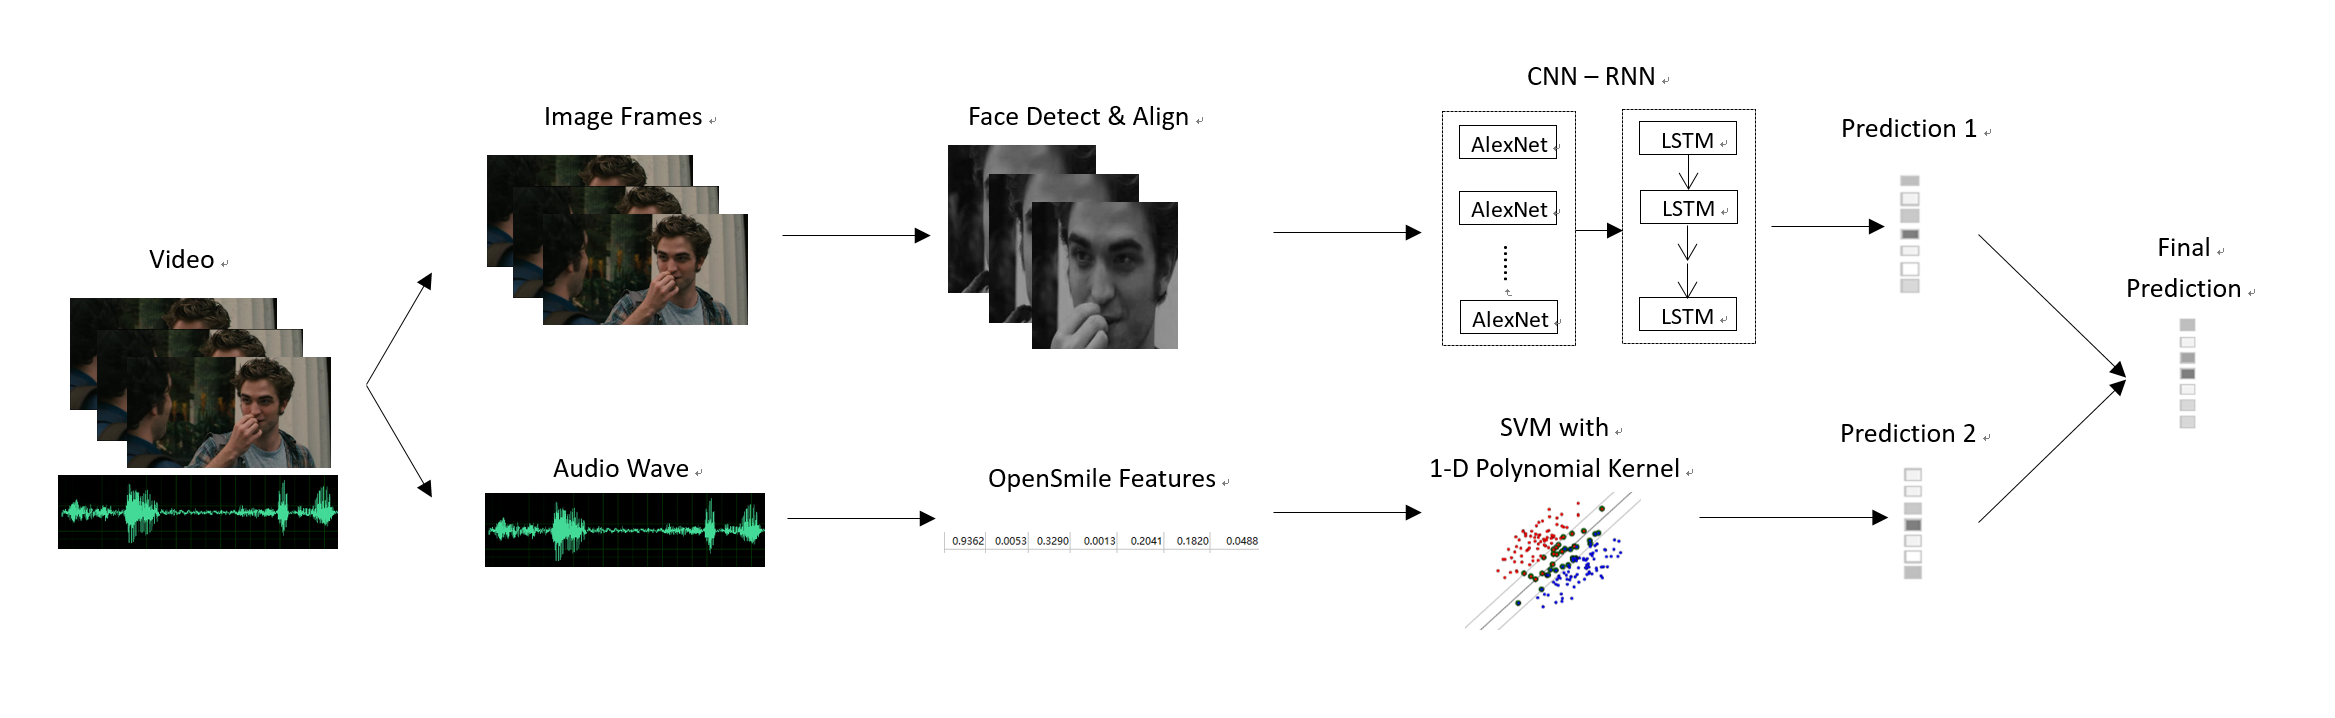
\includegraphics[width = \textwidth]{pic/pipeline.png}
	\caption{Pipeline}
\end{figure*}

\section{Intorduction}

Automatic emotion recoginition in videos has always been a field of major concern in the field of machine learning, particularly with the advancement of deep learning techniques. Emotion-aware systems are potentially capable of effectively analyzing human emotions and behaviors, and better serve our purposes in all sorts of applications.
While traditional machine learning methods, typically Support Vector Machines (SVM) are still popular around and continue to be used, deep learning methods which employ the artificial neural network are gaining increasingly wide applications for their impressive capabilities, such as the recent defeat of 50 world-class Go masters to the AI ``master''.

For the specific problem of video-based emotion recognition, an intuitive idea is to exploit both the visual frames and audio waves, and synthesize them together. Therefore as shall be demonstrated in the following sections, we set up two models for frames and audio respectively, with feature extraction and prediction. Please refer to the following sections for details. 

\section{Preprocessing}

For the visual part, it could be easily observed that there exists a large amount of unrelated information such as background, illumination, color, etc. that we humans do not need to reference while deciding a person's emotion. Thus, it would be reasonable that we conduct preprocessing procedure before feeding frames into neural network. Here we perform face detection and face alignment, which is a common process in tasks like face verification.

In face detection part, we tested two open source software. Openface \cite{amos2016openface} is a Python and Torch implementation of face recognition with deep neural networks and is based on the CVPR 2015 paper FaceNet \cite{schroff2015facenet}. A sad news is that its detection toolkit is currently developed on dlib \cite{king2009dlib}, which couldn't support CUDA, resulting in a huge time cost. One remedy we attempted on this software is to use thread pool parallel computing. By applying 8 threads concurrently we are able to compress the detection time of a video clip into 2 seconds or so. However, this software has another big issue that is basically not tolerable, detection recall.

Thus we found a more state of the art implementation of face detection, named Joint Face Detection and Alignment using Multi-task Cascaded Convolutional Neural Networks \cite{7553523}. It's a matcaffe implementation, which fits our environment quite well. More importantly, its detection recall is far more satisfying, so that we use this tool in our final submission. We provide our detection recall test result in Table 1. Not detected means not a single face was detected among all frames. 

\begin{table}[htpb]
	\begin{center}
		\begin{tabular}{|l|c|c|}
			\hline
			Method & Not Detected & Total Frames\\
			\hline\hline
			OpenFace & 75 & 383\\
			\hline
			MTCNN & 4 & 383\\
			\hline
		\end{tabular}
	\end{center}
	\caption{Detection results tested on Val set}
\end{table}

Since MTCNN was originally designed to generate detection and alignment result simultaneously, it is quite intuitive to apply affine transformation given 5 facial landmarks.


\section{Learn Visual Signals}

Visual signal is very important in emotion recognition. After preprocessing of the raw video, we obtain gray scale face series, which can be used for deep learning based method. Since the raw data is a video, it is a very straight-forward to apply CNN-RNN architecture to generate predictions. Considering the limited data and space limitation, we chose pretrained AlexNet, Inception-v2 and the CNN model trained with Center Loss from \cite{wen2016discriminative} for experiments. The first 2 models are pretrained on ImageNet and the last one was taken from the public code of the paper. As for RNN, we chose LSTM implemented in the standard Caffe.

\section{Learn Audio Signals}

Audio signal serves as another key component in video recognition. In the case of AFEW, it is found that audio segments from movie clips vary significantly within the dataset, e.g. the existence of speech and background music. Therefore, we predict the audio recognition result to be less accurate than the video dimension. Nonetheless, a proper exploitation of audio features can also provide reference to our recognition and improve the performance.

Although this project is essentially deep-learning-based, the traditional approach of SVM is employed for the processing of audio, for the purpose of reducing the size of our model. After all, the less satisfactory accuracy of audio makes it less worthwhile to occupy a large space.

We adopt the Opensmile toolbox \cite{eyben2010opensmile} for audio feature extraction. The feature configuration applied here is \texttt{emobase2010}, which projects each wave file onto a 1583-dimension vector, with features including loudness, MFCC values, etc. Since OpenSmile is most conveniently called with the WAV input format, we first reformat the AVI files into WAV audios with the \texttt{ffmpeg} tool. Both format transformation and feature extraction are conducted using system call. 

After acquiring the 1583-dimensional audio features, we apply an SVM classifier for recognition, the idea of which is insipired by the work of \cite{fan2016video}. Because that the methodology of SVM is intrinsically binary (two-class), certain tricks need to be employed for our task of seven-class classification. The LibSVM \cite{CC01a} toolbox implements multi-class SVM by multiple one-to-one SVMs, resulting in $n(n-1)/2$ SVMs for n-class classification, and consequently $n(n-1)/2$ decision values. For our purpose of a fusion of SVM and CNN predictions, we wish to reformulate the decision values into a 7-dimension vector. The method we designed is introduced as follows. For each class, we select the 6 relevent decision values out of the 21, decide the sign (positive or negative), take the exponential, then sum them up. This value after normalization gives the predicted probability which we require.

In the selection of SVM parameters, we experimented with several types of kernel functions including linear, polynomial and RBF. For each type of kernel, the choice of optimal parameters such as cost and weight are found using grid search method. The optimal prediction results on validation set is listed in table \ref{tableSVM}. It can be discovered that polynomial kernel with degree 1 yields the best performance. 

\begin{table}[htpb]
   \begin{center}
      \begin{tabular}{|c|c|}
         \hline
         \textbf{Kernel Type} & \textbf{Optimal Accuracy}\\
         \hline\hline
         Linear & 26.6\\
         \hline
         Polynomial $d$=1 & \textbf{31.3} \\
         \hline
         Polynomial $d$=2 & 24.5 \\
         \hline
         Polynomial $d$=3 & 22.7 \\
         \hline
         RBF & 16.7 \\
         \hline
         Sigmoid & 16.7 \\
         \hline
      \end{tabular}
   \end{center}
   \caption{Optimal SVM accuracy tested on Val set}
   \label{tableSVM}
\end{table}

\section{Model Fusion}

Referencing previous studies, prediction accuracy given by audio models are usually worse than video models, but it could be taken as decent feature supplement to video model, which usually results in an increase in model performance.

Here's what we do, we performance softmax manipulation on both video and audio outputs and get two probability distributions. We model our final probability prediction by function

\begin{equation}
Prob_{final} = Prob_{video} + t \times Prob_{video} 
\end{equation}

We selected the value of $t$ by investigating the performance of $t$ from $0$ to $1$ with a step of $0.01$ and got the curve shown in . From the figure we decided to choose the t value as $t=0.22$. The argmax of $Prob_{final}$ will serve as our final prediction.

Another implementation worth clarifying is that our audio model will always have a prediction while the video model will fail to do so if there's not a single face detected by MTCNN. In this case, we'll produce results solely by audio model, which is still higher than random guess. And from Table 1. we can see that this detection model rarely fails. 

\section{Experiment}

\subsection{Two-Step Fine-tuning}

Since the data in AFEW is quite limited, it is infeasible to directly fine-tune the models from ImageNet on it. So we take the 2-step fine-tuning strategy as in some state-of-the-art papers. Firstly we fine-tune our model on FER, which is another popular dataset for emotion recognition. Then we continue to fine-tune the model on AFEW

\subsection{Selection of Models}

We propose 3 candidate network models above, AlexNet, Inception-V2 and CenterLoss trained models. Firstly we fine-tune them on FER and select a model based on the performance on AFEW to show their generalization ability. The video accuracy was done by mean pooling the accuracies of each frame. The results are shown in Table \ref{tableSel}


\begin{table}[t]
\begin{center}
\vspace*{5pt}
\begin{tabular}{|c|c|c|}
\hline
\textbf{Model} & \textbf{Frame Accuracy} & \textbf{Video Accuracy} \\
\hline\hline
AlexNet & 27.6 & \textbf{29.0} \\
Inception-V2 & \textbf{27.8} & 28.2 \\
CenterLoss & 21.3 & 20.5 \\ 
\hline
\end{tabular}
\end{center}
\caption{Performance comparison of different models trained on FER}
\label{tableSel}

\end{table}

From the result above we can see that AlexNet and Inception-V2 lead to similar performance, while CenterLoss model is comparatively poor in performance. One possible result for this is center loss somehow makes it hard for the pretrained model to be used for transfer learning. AlexNet is better in speed while Inception-V2 has much less parameters. So we decide to take these 2 models into formal training process.



\subsection{Training}

In the training process, we adopt SGD to optimize the neural network. We set base learning rate to 1e-4, momentum=0.9, weight-decay=0.0005, gamma=0.1, and take early-stop strategy according to validation performance.

As mentioned above, we first train the network on FER and then train on AFEW. The 2 datasets are both trained for every single frame using Softmax. After that, we use the model to train a LSTM on it. We chose clip length = 15 for the LSTM and lr\_mult=10. Then we train with similar settings as mentioned above.

It is worth noticing that we adopt many techniques to prevent overfitting. Since the dataset AFEW is quite small, the neural network may overfit to the training set very easily. To address this problem, we first apply DropOut with ratio 0.5 to the output of fully connected layers. We also manage to add some gaussian noise to the very last layers of the network to further improve its generalization ability. The results show that our method achieve significant improvement compared to original models.

\subsection{Results}

Firstly we consider the visual part. To dig the best out of our network models, we actually conducted massive experiments. However, due to the length of the report, we only present the best result on videos by mean-pooling here. We show 4 results for both single frames and whole videos in Table \ref{tableResult}. \textbf{Pretrained} refers to the pretrained ImageNet models. \textbf{FER} refers to fine-tuning the pretrained model on FER and test on AFEW. \textbf{AFEW} refers to further fine-tuning the model on AFEW. \textbf{LSTM} refers to adding a LSTM to the CNN after training on AFEW. From the 4 results we can see the improvement in performance step by step.



\begin{table}[t]
\begin{center}
\begin{tabular}{|c|c|c|}
\hline
\textbf{Model} & \textbf{Video} & \textbf{Frame} \\
\hline\hline
AlexNet Pretrained & 15.83 & 13.47 \\
AlexNet FER & 29.01 & 27.63 \\
AlexNet AFEW & 41.16 &  35.32 \\
AlexNet + LSTM & 42.48 & 39.26  \\ 
\hline \hline 
Inception Pretrained & 13.19 & 14.21 \\
Inception FER & 28.21 & 27.80 \\
Inception AFEW & 44.06 & 37.43 \\
\textbf{Inception + LSTM} & \textbf{45.38} & \textbf{43.48} \\



\hline
\end{tabular}
\end{center}
\caption{Performance comparison of different models on AFEW. The results of Video are obtain by mean pooling every result of single frame.}
\label{tableResult}

\end{table}

Then we combine two domain models of best performance by fusion. We selected a value of $t$ as $0.22$, it could be seen from the figure that a relatively small $t$ ranges from $0.1$ to $0.3$ will usually have a facilitation effect.

\begin{figure}[htpb]
	\centering
	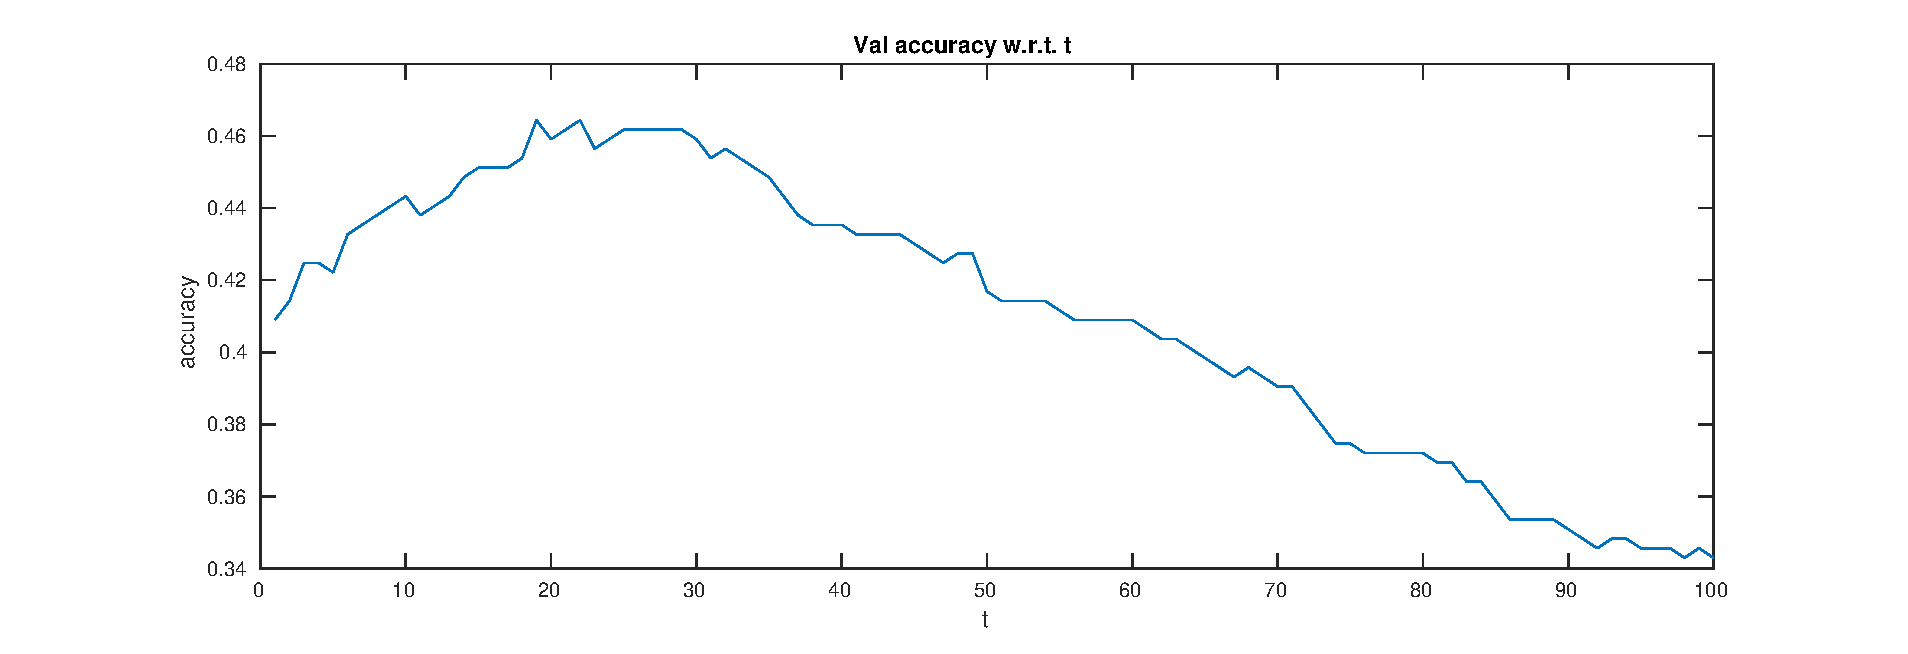
\includegraphics[width = 8cm]{pic/t_selection.eps}
	\caption{t selection curve}
\end{figure}

Here we perform our best result on validation set. We achieved an accuracy level of \textbf{47.23 \%}. From the confusion matrix we could see that the result is quite convincing, basically our model gives results to each class, though there are still some classes that this model performs not quite well.

\begin{figure}[htpb]
	\centering
	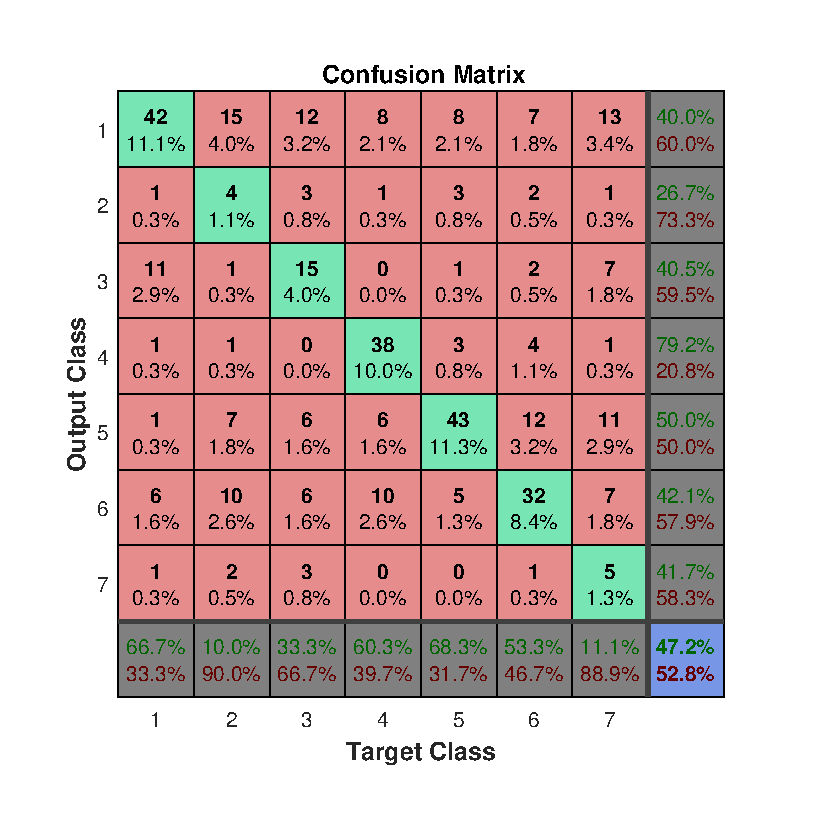
\includegraphics[width = 8cm]{pic/res_confusion.eps}
	\caption{confusion matrix}
\end{figure}

\subsection{Run Time Analysis}

We built our deploy version system on Ubuntu 14.04 with a GTX 970 GPU card and CPUs of Intel i7 core. From the table below we can see average time consumption of each part of the system.

\begin{table}[htpb]
	\begin{center}
		\begin{tabular}{|c|c|}
			\hline
			\textbf{Process} & \textbf{Time Cost Average} \\
			\hline\hline
			Video Preprocessing & 1.18s\\
			Audio Part in All &  0.25s \\
			CNN-LSTM (load model inside) &  2.88s \\
			
			
			\hline
		\end{tabular}
	\end{center}
	\caption{Run time analysys}
	\label{runtime}
	
\end{table}

Note that the two time costing parts will use GPU, which could be largely accelerated while replacing GTX 970 with TITAN X.

\section{Conclusion}

In this paper, we implemented a network for video-based emotion recognition in the wild, using CNN-LSTM and SVM, as a combination of deep learning and traditional learning methods. The results demonstrate that the combination of the two networks improves the prediction accuracy, which proves the effectiveness of the method.

\section{Acknowledgement}

Lin Ji trained all the image-based caffe models. Yan Jingkai has accomplished audio model. Cao Kaidi is responsible for video preprocessing, model fusion and deployment.

{\small
\bibliographystyle{ieee}
\bibliography{AFEW}
}

\end{document}
